\PassOptionsToPackage{pdfpagelabels=false}{hyperref} 
\documentclass[10pt, xcolor=x11names]{beamer}			% festlegen des dokumententyps

\usepackage{url}

\usepackage[utf8]{inputenc}
\usepackage[ngerman]{babel}
\usepackage{graphicx}
\usepackage{verbatim}


\usepackage{amssymb,amsfonts,amsmath,latexsym}

\usetheme{Copenhagen}
\usecolortheme{beaver}

\setbeamertemplate{navigation symbols}{}
\setbeamercolor{block title}{bg=red!80,fg=white}
\setbeamercovered{transparent}
\setbeamercolor{block body}{fg=black, bg=white!95!black}
\setbeamertemplate{navigation symbols}{}


\title{Built-Automation}
\subtitle{Gradle}
\author[S. Kuhnert und M. Thurner]{Stefan Kuhnert \and Thurner Michael}

\begin{document}

	\frame{\maketitle}
	
	\frame{\tableofcontents}
	
	\section{Was ist Gradle}
	\begin{frame}{Was ist Gradle}
		\begin{itemize}[<+->]
			\item Built-Automation Tool:
			\begin{itemize}[<+->]
				\item komplexe Projekte
				\item built-by-convention
			\end{itemize}
			\item Weiterentwicklung bestehender Systeme \(\rightarrow\) dazu später mehr
		\end{itemize}
	\end{frame}
	
	
	\section{Technik}
	\begin{frame}{Technik}
		\begin{itemize}[<+->]
			\item DSL \(\rightarrow\) auf groovy basierend
			\begin{itemize}[<+->]
				\item bessere Lesbarkeit
				\item direkt ausführbar
			\end{itemize}
			\item DAG:
			\begin{itemize}[<+->]
				\item Abarbeitungsreihenfolge der Tasks
			\end{itemize}
		\end{itemize}
	\end{frame}
	
	\section{Building}
	\begin{frame}{Building}
		\begin{itemize}[<+->]
			\item Parallelisierung:
			\begin{itemize}[<+->]
				\item Tasks können auf mehreren CPUs/Systemen laufen
			\end{itemize}
			\item Incremental Build:
			\begin{itemize}[<+->]
				\item nur bei Veränderung
			\end{itemize}
			\item Build-Prozess:
			\begin{itemize}[<+->]
				\item Konfiguration
				\item Ausführung
			\end{itemize}
		\end{itemize}
	\end{frame}
	
	\section{Aspekte anderer Systeme}
	\begin{frame}{Aspekte anderer Systeme}
		\begin{itemize}[<+->]
			\item ANT
			\begin{itemize}[<+->]
				\item Flexibilität
				\item Kontrolle
			\end{itemize}
			\item Ivy
			\begin{itemize}[<+->]
				\item Abhängigkeitsmanagement
			\end{itemize}
			\item Maven
			\begin{itemize}[<+->]
				\item Convention over configuration
				\item Multimodulare Projekte
				\item erweiterbar durch Plugins
			\end{itemize}
			\item GANT
			\begin{itemize}[<+->]
				\item Groovy-DSL
			\end{itemize}
		\end{itemize}
	\end{frame}

	\section{Frameworks}
	\begin{frame}{Frameworks}
		\begin{itemize}[<+->]
			\item Gradle wird von folgenden Frameworks verwendet:
			\begin{itemize}[<+->]
				\item Hibernate (relationale DB)
				\item Grails (Web App für Groovy)
				\item Groovy
				\item Spring (Java)
				\item Android
			\end{itemize}
		\end{itemize}

	\end{frame}

	
	
	\section{Beispiel}
	\begin{frame}{Beispiel}{Unser Server-Gradle Script}
		\begin{center}
		       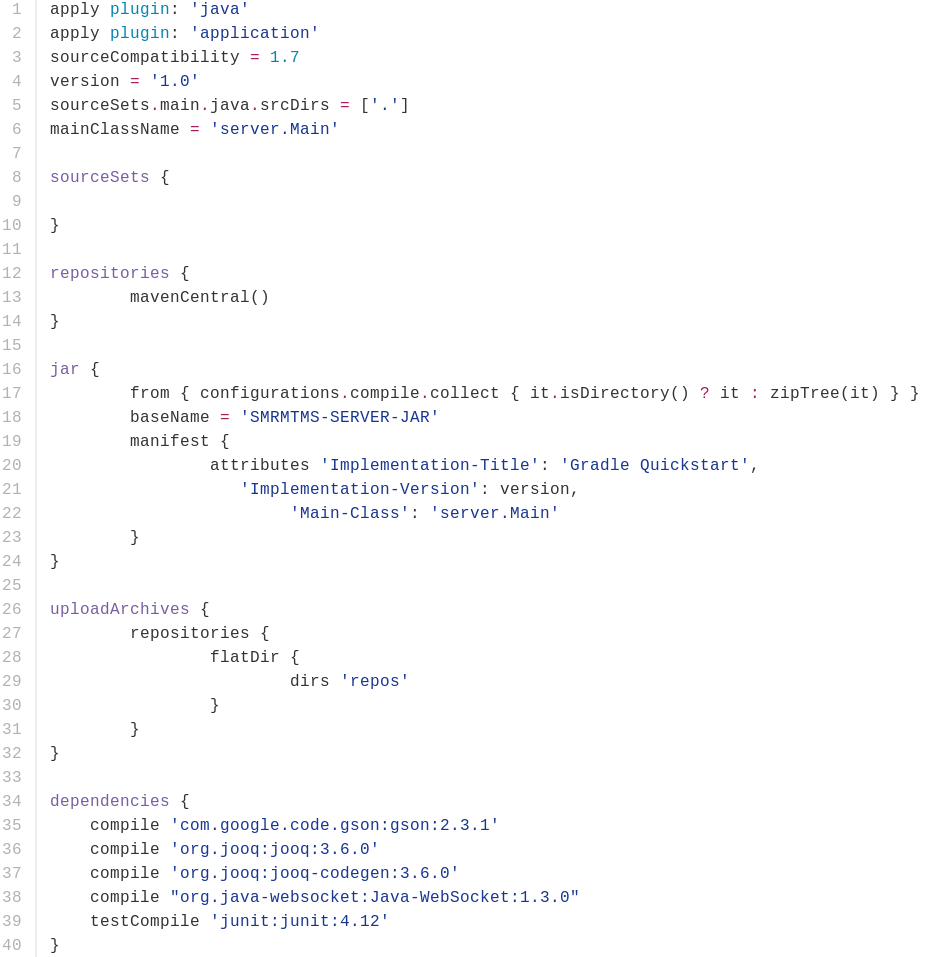
\includegraphics[width=\textwidth,height=\textheight,keepaspectratio]{gradle.png}
		\end{center}
	\end{frame}

\end{document}
